\section{Auswertung}

Der Relaxationsstroms wird für zwei verschiedene Heizraten (\SI{1.5}{\kelvin\per\minute} und \SI{2.0}{\kelvin\per\minute}) in Abhängigkeit der Temperatur gemessen. Aus dem Strom werden die Aktivierugnsenergie und die Relaxationszeit bestimmt. Fehler und Ausgleichsrechnungen werden mit den Python-Paketen SciPy \cite{scipy} und uncertainties \cite{uncertain} berechnet.

\subsection{Untergrundsubtraktion}

Die Messdaten müssen zunächst von einem Untergrund bereinigt werden. Dieser Untergrund ist das Resultat der steigenden Temperatur, was dazu führt, dass sich mehr Ladungsträger im Kristall bewegen können, was sich in einem kontinuierlichen Anstieg des gemessenen Stroms zeigt. Der Untergrund wird mit einem Polynom vierten Grades der Form
\begin{equation}
  I_\text{bg}(T) = aT^4 + bT^3 + cT^2 + dT + e
\end{equation}
modelliert. Die berechneten Parameter sind
\begin{equation*}
\begin{aligned}[c]
  \text{Heizrate: }& \SI{1.5}{\kelvin\per\minute}\\
  a &= \num{6.3(13)e-18}\\
  b &= \num{-6.2(14)e-15}\\
  c &= \num{2.3(5)e-12}\\
  d &= \num{-3.8(9)e-10}\\
  e &= \num{2.4(6)e-08}
\end{aligned}
\qquad
\begin{aligned}[c]
  \text{Heizrate: }& \SI{2.0}{\kelvin\per\minute}\\
  a &= \num{1.23(22)e-17}\\
  b &= \num{-1.20(23)e-14}\\
  c &= \num{4.4(9)e-12}\\
  d &= \num{-7.1(15)e-10}\\
  e &= \num{4.3(9)e-08}\,,
\end{aligned}
\end{equation*}
die Messdaten, zusammen mit dem Fit für den Untergrund sind in \autoref{fig:bg} dargestellt. In \autoref{fig:no-bg} sind die Messdaten ohne Untergrund und ohne den Anstieg vom zweiten Relaxationsvorgang zu sehen.

\begin{figure}[htp]
    \centering
    \begin{subfigure}[t]{0.5\textwidth}
        \centering
        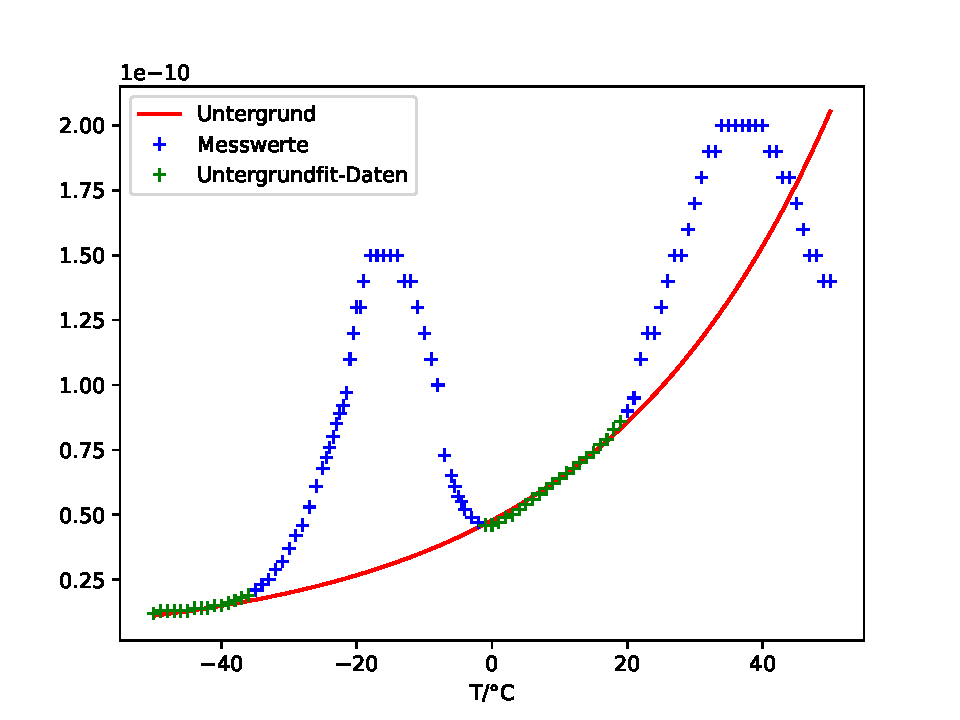
\includegraphics[width=\textwidth]{img/heizrate_15C.pdf}
        \caption{Heizrate: $\SI{1.5}{\kelvin\per\minute}$}
    \end{subfigure}%
    ~
    \begin{subfigure}[t]{0.5\textwidth}
        \centering
        \includegraphics[width=\textwidth]{img/heizrate_2C.pdf}
        \caption{Heizrate: $\SI{2.0}{\kelvin\per\minute}$}
    \end{subfigure}
    \caption{Temperaturabhängiger Verlauf der Messdaten und Fit an den Untergrund durch ein Polynom vierten Grades.}
    \label{fig:bg}
\end{figure}

\begin{figure}[htp]
    \centering
    \begin{subfigure}[t]{0.5\textwidth}
        \centering
        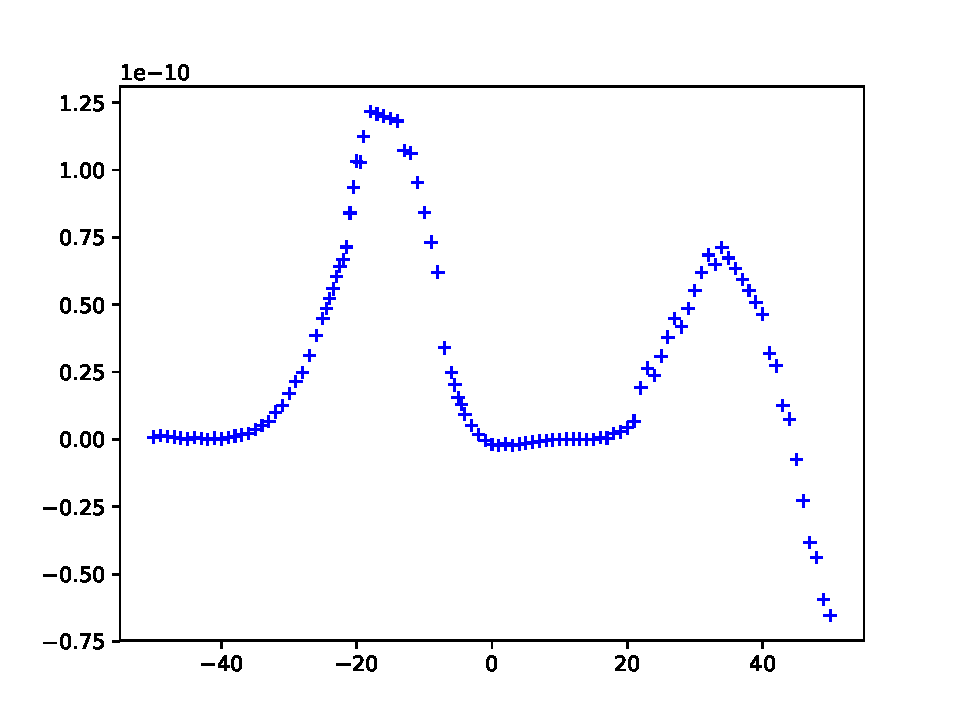
\includegraphics[width=\textwidth]{img/heizrate_15C_no-bg.pdf}
        \caption{Heizrate: $\SI{1.5}{\kelvin\per\minute}$}
    \end{subfigure}%
    ~
    \begin{subfigure}[t]{0.5\textwidth}
        \centering
        \includegraphics[width=\textwidth]{img/heizrate_2C_no-bg.pdf}
        \caption{Heizrate: $\SI{2.0}{\kelvin\per\minute}$}
    \end{subfigure}
    \caption{Vom Untergrund bereinigte und Messwerte ohne den zweiten Anstieg des Relaxationsstroms.}
    \label{fig:no-bg}
\end{figure}

Das Maximum im Relaxationsstrom ist für die beiden Heizraten
\begin{equation*}
\begin{aligned}[c]
  \text{Heizrate: }& \SI{1.5}{\kelvin\per\minute}\\
  T_\text{max} = \SI{255.15}{\kelvin}
\end{aligned}
\qquad
\begin{aligned}[c]
  \text{Heizrate: }& \SI{2.0}{\kelvin\per\minute}\\
  T_\text{max} = \SI{259.15}{\kelvin}\,,
\end{aligned}
\end{equation*}

\subsection{Bestimmung der Aktivierungsenergie durch einen linearen Fit}
\label{sec:lin}

Die erste Methode, mit der die Aktivierugnsenergie $W$ bestimmt wird, ist, indem eine Gerade an den linearen Verlauf des logarithmierten Stroms in Abhängigkeit von $1/T$ gefittet wird. Gemäß \autoref{eq:meth1} ist mit dem Fit
\begin{equation}
  \ln{(j(T))} = a \cdot \frac{1}{T} + b
\end{equation}
die Aktivierungsenergie
\begin{equation*}
  W_\text{meth1} = a \cdot k_\text{B}\,.
\end{equation*}
Die Fitparameter und daraus resultierende Aktivierugnsenergie und Relaxationszeit sind
\begin{equation*}
\begin{aligned}[c]
  \text{Heizrate: }& \SI{1.5}{\kelvin\per\minute}\\
  a &= \num{-1.388(33)e+04}\\
  b &= \num{32.1(14)}\\
  W &= \SI{1.196(29)}{\electronvolt}\\
  \tau_0 &= \SI{0.7(10)e-23}{\second}
\end{aligned}
\qquad
\begin{aligned}[c]
  \text{Heizrate: }& \SI{2.0}{\kelvin\per\minute}\\
  a &= \num{-9.61(30)e+03}\\
  b &= \num{15.0(12)}\\
  W &= \SI{0.829(26)}{\electronvolt}\\
  \tau_0 &= \SI{2.7(32)e-16}{\second}\,.
\end{aligned}
\end{equation*}
Die Relaxationszeit wird dabei mit \autoref{eq:tau0} bestimmt. Die ensprechenden Plot sind in \autoref{fig:meth1}.
\begin{figure}[htp]
    \centering
    \begin{subfigure}[t]{0.5\textwidth}
        \centering
        \includegraphics[width=\textwidth]{img/hr15_W-aus-Methode1.pdf}
        \caption{Heizrate: $\SI{1.5}{\kelvin\per\minute}$}
    \end{subfigure}%
    ~
    \begin{subfigure}[t]{0.5\textwidth}
        \centering
        \includegraphics[width=\textwidth]{img/hr2_W-aus-Methode1.pdf}
        \caption{Heizrate: $\SI{2.0}{\kelvin\per\minute}$}
    \end{subfigure}
    \caption{Bestimmung der Aktivierungsenergie $W$ durch einen linearen Fit an den Anstieg des Relaxationsstroms.}
    \label{fig:meth1}
\end{figure}

\subsection{Bestimmung der Aktivierungsenergie durch Integration}
\label{sec:linin}

\begin{figure}[htp]
    \centering
    \begin{subfigure}[t]{0.5\textwidth}
        \centering
        \includegraphics[width=\textwidth]{img/hr15_W-aus-Methode2.pdf}
        \caption{Heizrate: $\SI{1.5}{\kelvin\per\minute}$}
    \end{subfigure}%
    ~
    \begin{subfigure}[t]{0.5\textwidth}
        \centering
        \includegraphics[width=\textwidth]{img/hr2_W-aus-Methode2.pdf}
        \caption{Heizrate: $\SI{2.0}{\kelvin\per\minute}$}
    \end{subfigure}
    \caption{Bestimmung der Aktivierungsenergie $W$ durch einen linearen Fit an die gewichtete Integration des gesamten Verlaufs des Relaxationsstroms.}
    \label{fig:meth2}
\end{figure}

Eine genauere Bestimmung der Aktivierungsenergie $W$ erfolgt anhand \autoref{eq:meth2}. Dazu wird die integrierte und gewichtete Stromdichte linear gegen $1/T$ aufgetragen und die Fitparameter bestimmt. Die Aktivierungsenergie ist dann mit der Steigung $a$ der Gerade
\begin{equation*}
    W = a \cdot k_\text{B}\,.
\end{equation*}
Die Werte sind
\begin{equation*}
\begin{aligned}[c]
  \text{Heizrate: }& \SI{1.5}{\kelvin\per\minute}\\
  a &= \num{1.158(33)e+04}\\
  b &= \num{-42.7(13)}\\
  W &= \SI{0.998(29)}{\electronvolt}\\
  \tau_0 &= \SI{0.7(10)e-19}{\second}
\end{aligned}
\qquad
\begin{aligned}[c]
  \text{Heizrate: }& \SI{2.0}{\kelvin\per\minute}\\
  a &= \num{1.011(18)e+04}\\
  b &= \num{-36.8(7)}\\
  W &= \SI{0.871(15)}{\electronvolt}\\
  \tau_0 &= \SI{3.8(26)e-17}{\second}
\end{aligned}
\end{equation*}
und die Plots sind in \autoref{fig:meth2} zu sehen.

\subsection{Temperaturabhängiger Verlauf der Relaxationszeit}

In \autoref{fig:tau} ist der temperaturabhängige Verlauf der Relaxationszeit für beide Heizraten zu sehen, dazu wurde \autoref{eq:tau} verwendet. Pro Heizrate sind zwei Kurven dargestellt, da die Ergebnisse der in \autoref{sec:lin} und \autoref{sec:linin} verwendeteten Methoden gegenübergestellt werden.

\begin{figure}[htp]
    \centering
    \begin{subfigure}[t]{0.5\textwidth}
        \centering
        \includegraphics[width=\textwidth]{img/hr15_tau.pdf}
        \caption{Heizrate: $\SI{1.5}{\kelvin\per\minute}$}
    \end{subfigure}%
    ~
    \begin{subfigure}[t]{0.5\textwidth}
        \centering
        \includegraphics[width=\textwidth]{img/hr2_tau.pdf}
        \caption{Heizrate: $\SI{2.0}{\kelvin\per\minute}$}
    \end{subfigure}
    \caption{Temperaturabhängiger Verlauf der Relaxationszeit; für die Relaxationszeit $\tau_0$ sind  pro Heizrate zwei Berechnungsmethoden angewandt worden.}
    \label{fig:tau}
\end{figure}
